\begin{figure}[htbp]
\centering
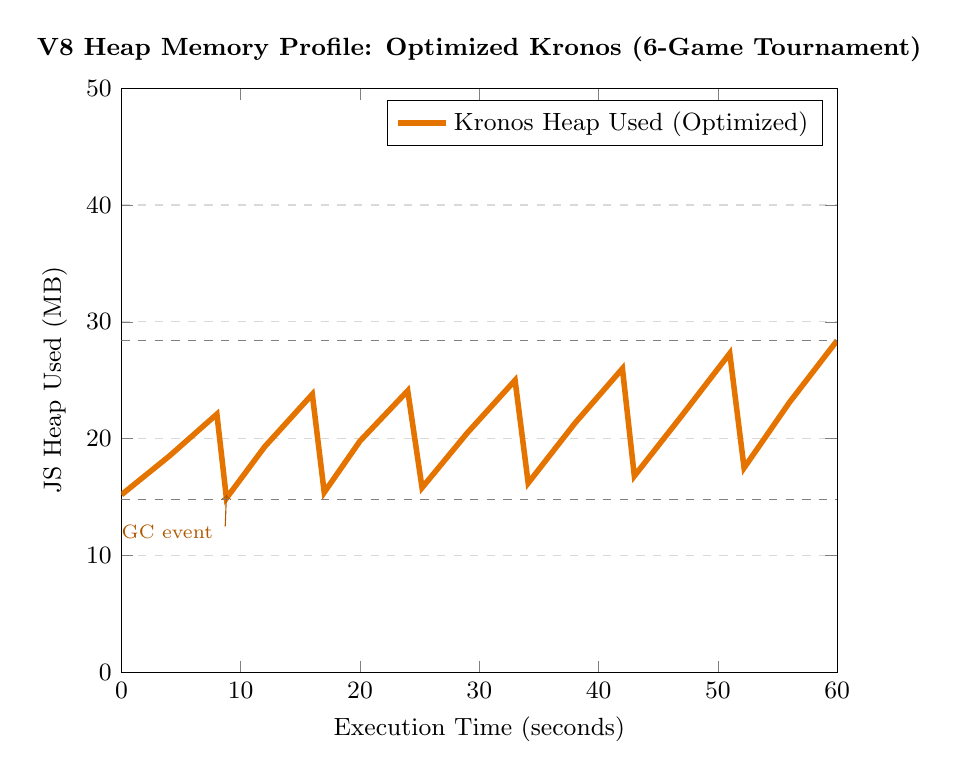
\begin{tikzpicture}
\begin{axis}[
    title style={font=\bfseries\small},
    title={V8 Heap Memory Profile: Optimized Kronos (6-Game Tournament)},
    xlabel={Execution Time (seconds)},
    ylabel={JS Heap Used (MB)},
    xmin=0, xmax=60,
    ymin=0, ymax=50,
    ymajorgrids=true,
    grid style={dashed, gray!30},
    width=0.88\textwidth,
    height=9cm,
    tick label style={font=\small},
    label style={font=\small},
    legend style={font=\small}
]
% Stable optimized heap profile with minor GC teeth
\addplot[
    color=orange!90!black,
    line width=2pt
]
coordinates {
    (0,  15.2)
    (4,  18.5)
    (8,  22.1)
    (8.8, 14.9)   % GC event 1
    (12, 19.3)
    (16, 23.8)
    (17.0, 15.4)  % GC event 2
    (20, 19.8)
    (24, 24.1)
    (25.2, 15.8)  % GC event 3
    (29, 20.5)
    (33, 25.0)
    (34.1, 16.2)  % GC event 4
    (38, 21.3)
    (42, 26.0)
    (43.0, 16.8)  % GC event 5
    (47, 22.0)
    (51, 27.3)
    (52.2, 17.5)  % GC event 6
    (56, 23.1)
    (60, 28.4)
};
\addlegendentry{Kronos Heap Used (Optimized)}

% Annotate stable range
\draw[dashed, gray] (axis cs:0,14.8) -- (axis cs:60,14.8)
    node[right, font=\scriptsize, text=gray] {14.8 MB};
\draw[dashed, gray] (axis cs:0,28.4) -- (axis cs:60,28.4)
    node[right, font=\scriptsize, text=gray] {28.4 MB};

% Label a GC event
\node[font=\scriptsize, text=orange!70!black, anchor=east]
    at (axis cs:8.5, 12) {GC event};
\draw[->, orange!70!black, thin] (axis cs:8.7,12.5) -- (axis cs:8.8,15.2);

\end{axis}
\end{tikzpicture}
\caption[Heap Memory Usage during Tournament]{V8 heap memory profile during a 6-game tournament with the optimized Kronos engine. The sawtooth pattern reflects normal minor GC cycles; the heap remains bounded between 14.8\,MB and 28.4\,MB throughout. This stability prevents major GC sweeps.}

\label{fig:memory_usage}
\end{figure}
% Source Material: MEMORY_PROFILE.md — optimized tournament run telemetry
